% vim: ts=4 sts=4 sw=4 tw=80
\chapter{Vim 脚本基础}
\label{chap:basic_vim_scripting}
\marginpar{141}

Vim 的一个最强大之处是允许高级用户通过编写脚本来增强 Vim 的功能. 通过脚本, 用
户几乎可以往 Vim 中添加任意功能, 而且很容易与其他用户分享.

这一章将会介绍编写 Vim 脚本的基础知识, 讨论的主题包括:
\begin{itemize}
    \item 编写语法高亮脚本
    \item 安装与使用脚本
    \item 不同类型的脚本
    \item 如何开发脚本
    \item Vim 脚本的基本语法
    \item 在 Vim 脚本中使用其他脚本语言
\end{itemize}

学习完这一章之后, 对于如何使用 Vim 脚本, 读者应该会有一个基本的概念, 而且有能
力写出一个简单的脚本, 从而为 Vim 添加新的功能.

\section{语法高亮方案}
\label{sec:syntax_color_schemes}

在许多程序员看来, 根据语法来高亮代码是 Vim 最重要的特性之一. 语法高亮不仅使代码
看起来更清晰, 还可以帮助用户发现编码错误. Vim 语法高亮系统所使用的脚本非常像
Vim 脚本, 但是语法高亮脚本定义的是颜色, 而不是功能. 在下面的一节里, 我们将会介
绍如何创建一个语法高亮方案.
\marginpar{142}

\subsection{第一个语法高亮文件}
\label{subsec:your_first_syntax_color_file}

简单来说, 语法高亮的关键是识别出文本中的特定单词与结构, 然后再给它们设置上对
应的颜色. 然而, 大部分情况下要稍微复杂一点, 因为语法高亮还需要识别上下文语境.
假设我们现在要语法高亮下面的代码:
\begin{vimcode}
/* if x equals y then return the value */
if (x == y)
  {
    return x;
  }
\end{vimcode}

如果我们仅仅是根据单词与符号来匹配, 那也可以得到一个相当不错的结果. 下面是具体
的配置命令 (每个选项的意义已经在第 \ref{chap:personalizing_vim} 章中进行了介
绍):
\begin{vimcode}
:syntax keyword myVars x y
:syntax match mySymbols "[{}();=]"
:syntax keyword myKeywords if return
:highlight myVars ctermfg=red guifg=red
:highlight mySymbols ctermfg=blue guifg=blue
:highlight myKeywords ctermfg=green guifg=green
\end{vimcode}

\begin{center}
    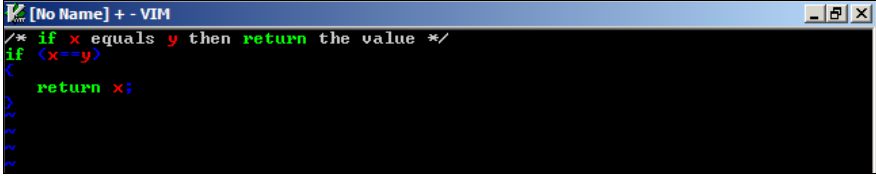
\includegraphics[scale=0.5]{./images/page142.png}
\end{center}

从上图中可以看到, 代码部分的高亮还不错, 可是注释语句却不令人满意. 这是因为我们
只是对单个单词进行匹配, 所以注释中的相同单词也会被匹配. 这种配置方法很难分辨出
代码与注释.
\marginpar{143}

那么, 我们可以从这个简单的例子里学习哪些东西呢? 那就是, 与高亮比起来, 更重要的
是要找到期望中的单词, 然后再给它们设置对应的颜色. 现在让我们增加一些上下文的信
息, 我们要把 \verb'/*' 与 \verb'*/' 之间的部分标记成注释, 然后再高亮其余的部
分. 代码部分被标记上颜色之后, 就不需要再上色了, 因此规则的顺序很重要. 具体的
配置代码是:
\begin{vimcode}
:syntax match myComments "/\*.*\*/"
:syntax keyword myVars x y
:syntax match mySymbols "[{}();=]"
:syntax keyword myKeywords if return
:highlight myVars ctermfg=red guifg=red
:highlight mySymbols ctermfg=blue guifg=blue
:highlight myKeywords ctermfg=green guifg=green
:highlight myComments ctermfg=yellow guifg=yellow
\end{vimcode}
最终的效果是:
\begin{center}
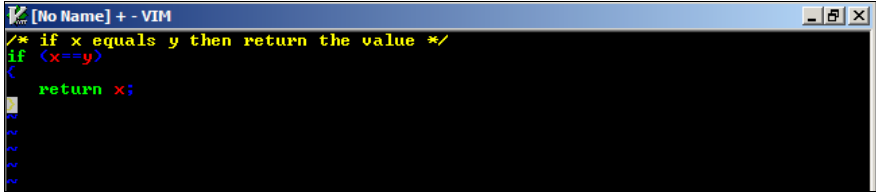
\includegraphics[scale=0.5]{./images/page143.png}
\end{center}

现在, 这段代码的高亮已经相当得体. 当然, 这只是一个小例子, 而且只用到了 Vim 语
法高亮的一小部分功能, 接下来, 我们将会介绍更多的内容.

\section{区域高亮}
\label{sec:syntax_regions}

在前面的例子中, 我们用的是选项 \texttt{match} 来选择注释语句. 在某些情况下,
我们很难创建一个适当的匹配语句, 这时候, 我们就需要用到其他一些更方便的做法.

在 Vim 中, 你可以选中一整个代码区, 然后再高亮它们, 为了选择一个代码区, 只需要
提供区域的开始与结束. 对于前面的例子, 如果使用区域高亮的话, 具体的命令是:
\begin{vimcode}
:syntax region myComments start=/\/\*/ end=/\*\//
\end{vimcode}
\marginpar{144}
